% =====================================================================
%  Introduction to Deep Learning — Class 25
%  Topic (course plan): Convolution Networks
%  Subtopic (course plan): Convolution Filters
%  Sources (course plan): Prince Chapter 10, Bishop Chapter 10
%
%  Class 23 defined the layer; Class 24 built three tasks on a trunk it
%  treated as given.  This class opens the trunk: how small filters
%  compose into large ones, what a standard architecture looks like
%  layer by layer, and what a trained filter turns out to respond to
%  — read off the weights, by maximising a unit, by differentiating
%  the output, and by turning the gradient against the network.
%
%  Order: stacking filters, a standard architecture, the visual cortex
%  and Gabor filters, learned filters and synthetic images, saliency,
%  adversarial attacks, DeepDream, style transfer.
%
%  A variant: every figure is the published one, cited on the slide.
%  See _shared/PLAN_Classes23_24_25.md.
%
%  Compile:  xelatex main.tex   (run twice)
% =====================================================================
\documentclass[aspectratio=169, 11pt]{beamer}

\usetheme{metropoliscustom}

\usepackage{graphicx}
\DeclareGraphicsExtensions{.pdf,.png,.jpg}
\graphicspath{{figs_official/}{Class25_Convolution_Filters_Learned/A_Textbook_Figures/figs_official/}}
\usepackage{amsmath, amssymb}
\usepackage{bm}
\usepackage{tikz}
\usetikzlibrary{arrows.meta, positioning, calc, decorations.pathreplacing,
                shapes.geometric, fit, backgrounds}
\tcbuselibrary{skins}

\definecolor{shc}{HTML}{341651}
\definecolor{tealc}{HTML}{1C7293}
\definecolor{dpc}{HTML}{800000}
\definecolor{accc}{HTML}{B8860B}

% ---- theorem environments -------------------------------------------
\setbeamertemplate{theorems}[numbered]
\usepackage{remreset}
\makeatletter\@removefromreset{theorem}{section}\makeatother
\renewcommand{\thetheorem}{\arabic{theorem}}
\newtheorem{lemmax}[theorem]{Lemma}
\newtheorem{propx}[theorem]{Proposition}
\newtheorem{corx}[theorem]{Corollary}
\newtheorem{defx}[theorem]{Definition}
\newtheorem{thmx}[theorem]{Theorem}

\newcommand{\bridge}[1]{%
  {\scriptsize\itshape\color{mcMuted} #1\par}\vspace{0.35em}}

\newcommand{\srcline}[1]{%
  \par\vspace{0.25em}%
  {\scriptsize\color{mcMuted}\hfill #1\par}}

\newcommand{\figsource}[1]{{\scriptsize\color{mcMuted} #1}}
\newcommand{\figcap}[2][0.90]{%
  \begin{center}\begin{minipage}{#1\textwidth}\centering
    {\scriptsize\color{mcMuted} #2}
  \end{minipage}\end{center}}

% =====================================================================
\title{Convolutional Networks}
\subtitle{Convolution Filters: What They Learn}
\author{Introduction to Deep Learning \ \textperiodcentered\ Class 25}
\institute{}
\date{}

\footleft{Introduction to Deep Learning}
\footright{What the Filters Learn}
\titlelogos{}

\begin{document}

\maketitle

\begin{frame}{Outline}
  \tableofcontents
\end{frame}

% =====================================================================
\section{Stacking Filters}
% =====================================================================

\begin{frame}{Opening the trunk}
  \bridge{Class 23 defined one layer. Class 24 built three tasks on a
  trunk it treated as a given. Today the trunk itself: how filters
  compose, what a standard one looks like, and what the filters turn
  out to detect.}
  \vspace{0.05em}
  {\scriptsize
  \renewcommand{\arraystretch}{1.30}
  \begin{tabular}{@{}l@{\hspace{1.4em}}l@{\hspace{1.4em}}l@{}}
    \textbf{Question} & \textbf{Tool} & \textbf{Where}\\
    how do small filters make big ones? & composition, receptive fields
      & \S10.2.7--10.2.8\\
    what does a standard trunk look like? & VGG-16, layer by layer &
      \S10.2.8\\
    what does a filter respond to? & the weights, maximising a unit,
      the gradient & \S10.3\\
    can the gradient be turned against it? & adversarial attacks,
      DeepDream & \S10.3.4--10.3.5\\
    what is style, to a network? & the style matrix & \S10.6\\
  \end{tabular}}
  \vspace{0.45em}

  \begin{redhighlight}
    One tool does most of the work today: the gradient of something
    the network computes, taken with respect to its \emph{input}.
  \end{redhighlight}
\end{frame}

\begin{frame}{Notation for today}
  \vspace{0.3em}
  {\footnotesize
  \renewcommand{\arraystretch}{1.30}
  \begin{columns}[T, onlytextwidth]
    \begin{column}{0.49\textwidth}
      \begin{tabular}{@{}l@{\hspace{1.4em}}l@{}}
        $M$ & kernel size, $M \times M$\\
        $C_{\mathrm{in}}$, $C_{\mathrm{out}}$ & channels in and out of a layer\\
        $\mathbf{W}_l$ & the kernel of layer $l$\\
        $a_{ijk}$ & pre-activation at $(i, j)$ of channel $k$\\
      \end{tabular}
    \end{column}
    \begin{column}{0.49\textwidth}
      \begin{tabular}{@{}l@{\hspace{1.4em}}l@{}}
        $a^{(c)}$ & pre-activation of output unit $c$\\
        $\mathbf{x}$ & the input image, as pixels\\
        $E(\mathbf{x}, t)$ & the error on $\mathbf{x}$ with true label $t$\\
        $\mathbf{F}$ & the style matrix, $K \times K$\\
      \end{tabular}
    \end{column}
  \end{columns}}
  \vspace{0.5em}

  \begin{itemize}\itemsep0.24em
    \item Bishop writes the filter tensor as
          $M \times M \times C_{\mathrm{IN}} \times C_{\mathrm{OUT}}$;
          Class 23 called the same object $\bm{\Omega}$ and the kernel
          size $k$
    \item Bishop reserves \emph{depth} for the number of layers; the
          number of channels is never called depth here
  \end{itemize}
  \srcline{Bishop \& Bishop (2024), \S10.2.7, \S10.3.}
\end{frame}

\begin{frame}{A layer, counted}
  \vspace{-0.25em}
  \begin{defx}[A convolutional layer with channels]\label{th:layer}
    \small
    A layer with $C_{\mathrm{in}}$ input channels and $C_{\mathrm{out}}$
    output channels, kernel $M \times M$, is a filter tensor of size
    $M \times M \times C_{\mathrm{in}} \times C_{\mathrm{out}}$ with
    \[
      (M^2 C_{\mathrm{in}} + 1)\, C_{\mathrm{out}}
    \]
    independent weights and biases. Its $C_{\mathrm{out}}$ output channels
    are the input channels of the next layer, as the RGB channels were
    of the first.
  \end{defx}
  \vspace{0.15em}
  {\footnotesize
  \begin{itemize}\itemsep0.22em
    \item Stack such layers, with optional pooling between, and the
          effective receptive field of a unit grows with every layer:
          Class 23 measured it
    \item The final fully connected layers see the whole image and may
          hold most of the \emph{parameters}, even though most of the
          \emph{connections} are convolutional
  \end{itemize}}
  \srcline{Bishop \& Bishop (2024), \S10.2.7, Fig.~10.9.}
\end{frame}

\begin{frame}{Reach grows with depth}
  \begin{center}
    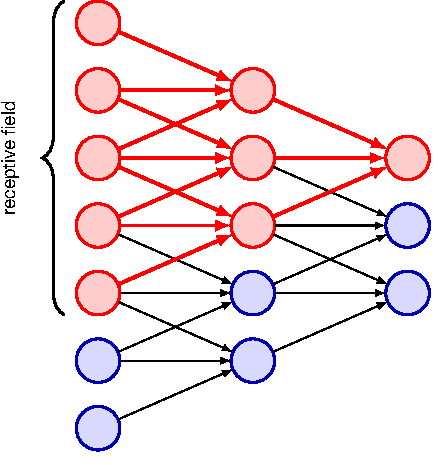
\includegraphics[height=0.50\textheight]{Bishop10_9}
  \end{center}
  \vspace{-0.2em}
  \figcap[0.97]{The red unit at the top reads three units of the middle
  layer, each of which reads three of the first, so it depends on five
  inputs: the effective receptive field grows with every layer, and a
  stack of small kernels reaches as far as one large kernel for fewer
  parameters. Bishop \& Bishop (2024), Fig.~10.9.}
\end{frame}

\begin{frame}{Two small filters are one large one --- until a ReLU}
  \vspace{-0.3em}
  \begin{propx}[Composition of kernels]\label{th:compose}
    \small
    Two convolutions in succession with kernels $\mathbf{W}_1$
    ($k_1 \times k_1$) and $\mathbf{W}_2$ ($k_2 \times k_2$), with no
    nonlinearity between them, equal one convolution with a kernel of
    size $(k_1 + k_2 - 1)^2$, namely $\mathbf{W}_2 * \mathbf{W}_1$. With a
    ReLU between them they are, in general, no single kernel at all.
  \end{propx}
  \vspace{0.05em}
  {\footnotesize
  \begin{itemize}\itemsep0.24em
    \item \focus{1}{Proof. Both operations are linear and
          translation-equivariant (Class 23), so their composition is
          too, and by the converse there it is a convolution; its
          kernel is the response to a single one, which is
          $\mathbf{W}_2 * \mathbf{W}_1$. \hfill $\square$}
    \item \focus{2}{So the stack of (a) is not only cheaper than the
          big kernel: it is \alert{constrained} to big kernels that
          factor into small ones --- an inductive bias, in Class 18's
          sense.}
    \item \focus{3}{The ReLU between layers is what makes depth more
          than a factorisation: the second filter reads a rectified
          map, and the whole is not linear in the image.}
  \end{itemize}}
  \vspace{-0.3em}
  \srcline{Bishop \& Bishop (2024), \S10.2.8; Class 23, the
  equivariance theorem.}
\end{frame}

\begin{frame}{The $1 \times 1$ convolution}
  \vspace{-0.3em}
  \begin{defx}[$1 \times 1$ convolution]\label{th:onebyone}
    \small
    A layer with $M = 1$: every output channel at position $(i, j)$ is
    a weighted sum of all input channels \emph{at that position}, plus
    a bias, through the activation function,
    \[
      z_{ijc'} = h\Big( \textstyle\sum_{c} w_{cc'}\, x_{ijc} + b_{c'} \Big),
    \]
    with $C_{\mathrm{in}} C_{\mathrm{out}} + C_{\mathrm{out}}$ parameters and no
    spatial mixing at all.
  \end{defx}
  \vspace{0.2em}
  {\footnotesize
  \begin{itemize}\itemsep0.24em
    \item It changes the number of channels without touching the
          resolution: the same linear map applied at every pixel
    \item Class 24 used it at the end of a segmentation network to
          turn feature channels into $C$ class scores; it is also how
          a trunk is made narrower between expensive layers
  \end{itemize}}
  \srcline{Prince (2023), \S10.5.1, Fig.~10.14.}
\end{frame}

% =====================================================================
\section{A Standard Architecture}
% =====================================================================

\begin{frame}{VGG-16, layer by layer}
  \vspace{0.05em}
  {\scriptsize
  \renewcommand{\arraystretch}{1.24}
  \begin{tabular}{@{}l@{\hspace{1.2em}}l@{\hspace{1.2em}}l@{\hspace{1.2em}}l@{}}
    \textbf{Stage} & \textbf{Layers} & \textbf{Output} & \textbf{Note}\\
    input & --- & $224 \times 224 \times 3$ & RGB\\
    block 1 & $2 \times$ conv $3 \times 3$, $64$ ch; pool &
      $112 \times 112 \times 64$ & first layer: $28$ parameters per filter\\
    block 2 & $2 \times$ conv, $128$ ch; pool & $56 \times 56 \times 128$ &
      channels double as the side halves\\
    blocks 3--5 & $3 \times$ conv each, $256 / 512 / 512$ ch; pool &
      $7 \times 7 \times 512$ & $25{,}088$ units at the end\\
    head & FC $4096$, FC $4096$, FC $1000$ & $1000$ & softmax at the end\\
  \end{tabular}}
  \vspace{0.2em}

  {\footnotesize
  \begin{itemize}\itemsep0.16em
    \item Three design rules and almost no other choices: every kernel
          $3 \times 3$, stride $1$, same padding, ReLU; every pooling
          $2 \times 2$, stride $2$; channels doubled after each pooling
          so the representation does not shrink too fast
    \item $16$ learnable layers; roughly $138$ million parameters,
          nearly $103$ million of them in the first fully connected layer
  \end{itemize}}
  \srcline{Bishop \& Bishop (2024), \S10.2.8, Fig.~10.10;
  Simonyan \& Zisserman (2015).}
\end{frame}

\begin{frame}{VGG-16, drawn}
  \begin{center}
    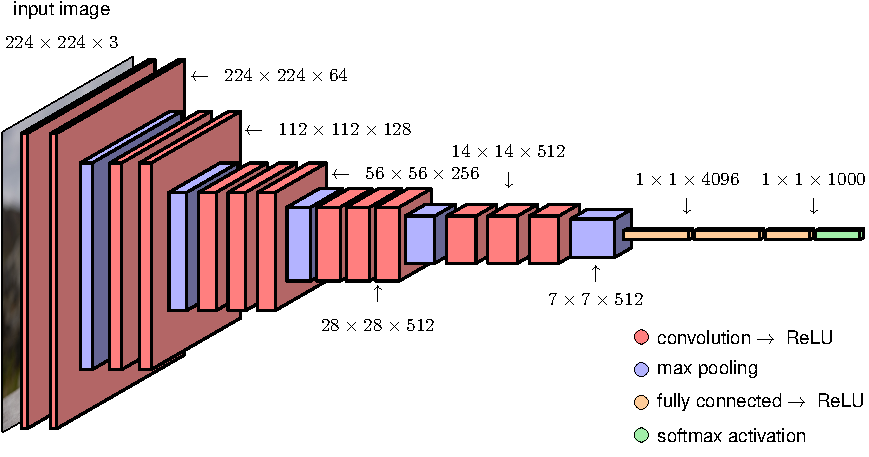
\includegraphics[width=0.60\linewidth]{Bishop10_10}
  \end{center}
  \vspace{-0.3em}
  \figcap[0.97]{Five blocks of $3 \times 3$ convolutions and
  $2 \times 2$ pooling to $7 \times 7 \times 512$, then three fully
  connected layers and a softmax; $138$ million parameters, nearly
  $103$ million in the first fully connected layer. Bishop \& Bishop
  (2024), Fig.~10.10.}
\end{frame}

\begin{frame}{What ImageNet did to the field}
  \vspace{0.1em}
  {\footnotesize
  \begin{itemize}\itemsep0.30em
    \item Convolutional networks were the first deep networks to work
          in applications: LeNet read handwritten digits in 1989
    \item ImageNet: some $14$ million labelled images in nearly
          $22{,}000$ categories; the challenge subset has $1{,}000$ and
          random guessing would score $99.9\%$ error
    \item Top-5 error: about $25.5\%$ before; $15.3\%$ for AlexNet in
          2012, with ReLUs, GPUs and dropout (Prince reports $16.4\%$);
          about $3\%$ later, past the $5\%$ or so of humans
    \item The lesson Bishop draws is not only depth: large data and a
          model with the \alert{right inductive bias} together
  \end{itemize}}
  \vspace{-0.1em}
  \begin{redhighlight}
    The trunk is a hypothesis about images, and ImageNet was large
    enough to reward it.
  \end{redhighlight}
  \vspace{-0.3em}
  \srcline{Bishop \& Bishop (2024), \S10.2.8; Prince (2023), \S10.5.1.}
\end{frame}

% =====================================================================
\section{What a Filter Responds To}
% =====================================================================

\begin{frame}{The visual cortex}
  \vspace{0.1em}
  {\footnotesize
  \begin{itemize}\itemsep0.28em
    \item Hubel and Wiesel (1959) recorded single neurons in the visual
          cortex of cats while showing them stimuli
    \item \alert{Simple cells} fire for an edge at one orientation and
          one position, and little else; their response is modelled by
          a Gabor filter
    \item \alert{Complex cells} combine simple cells and are partly
          invariant to small shifts --- the role pooling plays in a
          convolutional network
    \item Deeper cells are more specific and more invariant still; the
          notional \emph{grandmother cell} fires for one person at any
          location, scale or lighting
    \item The neocognitron (Fukushima, 1980) copied this: local
          receptive fields, shared weights, local pooling --- but no
          end-to-end training, since it predated backpropagation
  \end{itemize}}
  \srcline{Bishop \& Bishop (2024), \S10.3.1.}
\end{frame}

\begin{frame}{The Gabor filter}
  \vspace{-0.3em}
  \begin{defx}[Gabor filter]\label{th:gabor}
    \small
    \[
      G(x, y) = A \exp\!\big( -\alpha \tilde{x}^2 - \beta \tilde{y}^2 \big)
                \sin\!\big( \omega \tilde{x} + \phi \big),
      \qquad
      \begin{aligned}
        \tilde{x} &= (x - x_0)\cos\theta + (y - y_0)\sin\theta,\\
        \tilde{y} &= -(x - x_0)\sin\theta + (y - y_0)\cos\theta.
      \end{aligned}
    \]
  \end{defx}
  \vspace{0.05em}
  {\footnotesize
  \begin{itemize}\itemsep0.22em
    \item $(\tilde{x}, \tilde{y})$ is the coordinate system rotated by
          $\theta$, so the sine is a spatial oscillation in the
          direction $\theta$ with frequency $\omega$ and phase $\phi$
    \item The exponential is a decay envelope that localises the
          filter around $(x_0, y_0)$, with rates $\alpha$ and $\beta$
    \item Correlate an image with it and the response is large where
          there is an edge or a stripe at that orientation and scale,
          which is what a simple cell does
  \end{itemize}}
  \srcline{Bishop \& Bishop (2024), Eqs.~10.6--10.8, Fig.~10.11.}
\end{frame}

\begin{frame}{Gabor filters, drawn}
  \begin{center}
    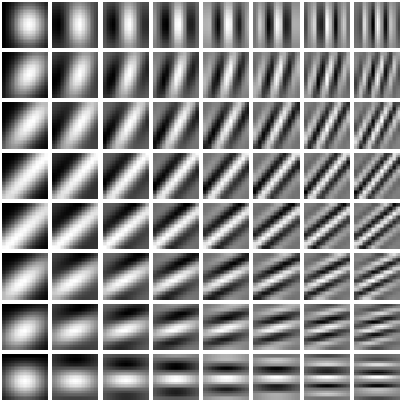
\includegraphics[height=0.56\textheight]{Bishop10_11}
  \end{center}
  \vspace{-0.2em}
  \figcap[0.97]{Eq.~10.6: the orientation $\theta$ runs from $0$ in the
  top row to $\pi/2$ in the bottom row, the frequency $\omega$ from $1$
  in the left column to $10$ in the right. Bishop \& Bishop (2024),
  Fig.~10.11.}
\end{frame}

\begin{frame}{Reading the first layer directly}
  \vspace{0.1em}
  {\footnotesize
  \begin{itemize}\itemsep0.30em
    \item A first-layer filter is a small patch in pixel space, so its
          weights can be shown as an image; the unit fires when the
          inner product with the patch under it is large
    \item The filters a network learns on ImageNet look remarkably like
          Gabor filters
    \item That is \emph{not} evidence that the network is a model of
          the brain: many statistical methods recover the same filters
          from natural images. They are a property of the
          \alert{statistics of images}, useful to any system that looks
          at them
    \item Deeper layers cannot be read this way: their inputs are
          filter responses, not pixels
  \end{itemize}}
  \srcline{Bishop \& Bishop (2024), \S10.3.2, Fig.~10.12;
  Hyv\"arinen et al.\ (2009).}
\end{frame}

\begin{frame}{The first layer of AlexNet}
  \begin{center}
    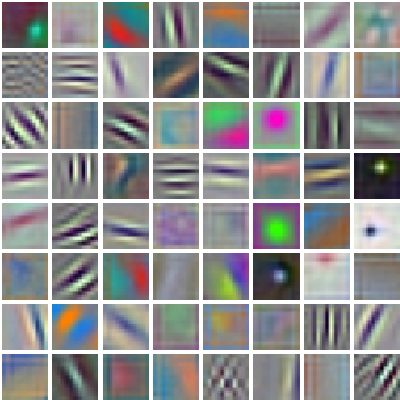
\includegraphics[height=0.58\textheight]{Bishop10_12}
  \end{center}
  \vspace{-0.3em}
  \figcap[0.97]{Learned first-layer filters of AlexNet: oriented edges
  and stripes at several scales, and colour-opponent blobs --- many of
  them Gabor filters to the eye. Bishop \& Bishop (2024), Fig.~10.12.}
\end{frame}

\begin{frame}{Deeper layers: ask what excites a unit}
  \vspace{0.1em}
  {\footnotesize
  \begin{itemize}\itemsep0.30em
    \item Hubel and Wiesel's method, applied to a network: show it many
          image patches and keep the ones that excite a given unit most
    \item Doing this for a five-layer network trained on ImageNet
          shows a \alert{hierarchy}: edges in layer 1, textures and
          simple shapes in layer 2, parts of objects in layer 3, whole
          objects in layer 5
    \item The same locality and pooling that gave Class 23's growing
          receptive field give this growing meaning
  \end{itemize}}
  \vspace{0.2em}
  \begin{redhighlight}
    Depth composes filters into detectors of larger and more abstract
    things, layer by layer --- what the composition proposition
    permits, and the ReLU makes non-trivial.
  \end{redhighlight}
  \srcline{Bishop \& Bishop (2024), \S10.3.2, Fig.~10.13;
  Zeiler \& Fergus (2013).}
\end{frame}

\begin{frame}{Patches that excite units, by layer}
  \begin{center}
    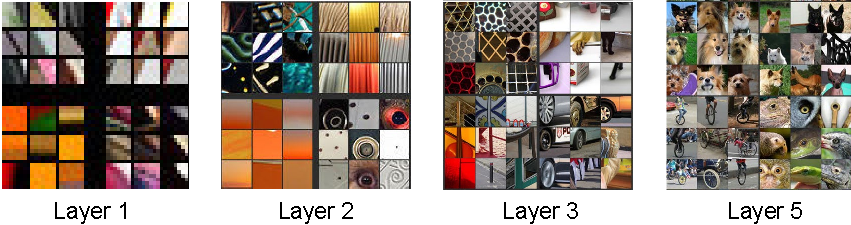
\includegraphics[width=0.92\linewidth]{Bishop10_13}
  \end{center}
  \vspace{-0.2em}
  \figcap[0.97]{For four channels in each of layers 1, 2, 3 and 5, the
  nine validation patches with the strongest activation, as a
  $3 \times 3$ grid each: edges, then textures, then object parts, then
  objects. Bishop \& Bishop (2024), Fig.~10.13, from Zeiler \& Fergus
  (2013).}
\end{frame}

\begin{frame}{Or optimise the image}
  \vspace{-0.45em}
  \begin{propx}[Maximise the pre-activation, not the probability]\label{th:preact}
    \small
    To find the image most representative of class $c$, ascend the
    pre-activation $a^{(c)}(\mathbf{x})$, not the softmax output $p_c$:
    \[
      \frac{\partial \log p_c}{\partial a^{(c')}} = \delta_{cc'} - p_{c'} ,
    \]
    so the gradient of $p_c$ depends on every other class through the
    denominator: it would make the image \emph{less} like a cat as much
    as more like a dog.
  \end{propx}
  \vspace{0.1em}
  {\footnotesize
  \begin{itemize}\itemsep0.22em
    \item Unconstrained ascent sends pixels to infinity, so it is
          regularised: a sum-of-squares penalty, blurring between steps,
          clipping of pixels that contribute little
    \item The result is a \alert{synthetic image} of the class; the
          same gradient, pointed the other way, is an attack
  \end{itemize}}
  \srcline{Bishop \& Bishop (2024), \S10.3.2, Fig.~10.14;
  Yosinski et al.\ (2015).}
\end{frame}

\begin{frame}{Synthetic images of four classes}
  \begin{center}
    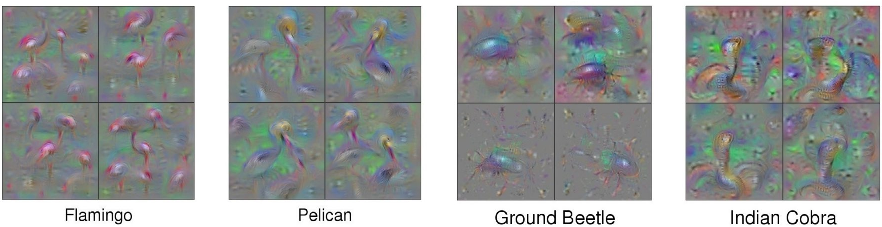
\includegraphics[width=0.92\linewidth]{Bishop10_14}
  \end{center}
  \vspace{-0.2em}
  \figcap[0.97]{Images that maximise a class output of a trained
  classifier, four regularisation settings per class. Bishop \& Bishop
  (2024), Fig.~10.14, from Yosinski et al.\ (2015).}
\end{frame}

% =====================================================================
\section{Reading and Fooling a Network}
% =====================================================================

\begin{frame}{Saliency: which pixels decided}
  \vspace{-0.3em}
  \begin{defx}[Grad-CAM]\label{th:gradcam}
    \small
    For an input image and a class $c$, take the last convolutional
    layer, with $M_k$ units in channel $k$ and pre-activations
    $a^{(k)}_{ij}$. Average the gradient of the class pre-activation over
    each channel, and weight the channels by it:
    \[
      \alpha_k = \frac{1}{M_k}\sum_i \sum_j
        \frac{\partial a^{(c)}}{\partial a^{(k)}_{ij}},
      \qquad
      \mathbf{L} = \sum_k \alpha_k \mathbf{A}^{(k)} .
    \]
  \end{defx}
  \vspace{0.1em}
  {\footnotesize
  \begin{itemize}\itemsep0.22em
    \item The last convolutional layer is the right place: it still has
          positions, which the fully connected layers lose, and the
          most semantic features
    \item $\mathbf{L}$ has the size of that layer --- $14 \times 14$ for
          VGG-16 --- and is drawn over the image as a heat map
  \end{itemize}}
  \vspace{-0.3em}
  \srcline{Bishop \& Bishop (2024), \S10.3.3, Eqs.~10.9--10.10;
  Selvaraju et al.\ (2016).}
\end{frame}

\begin{frame}{Saliency, on an image}
  \begin{center}
    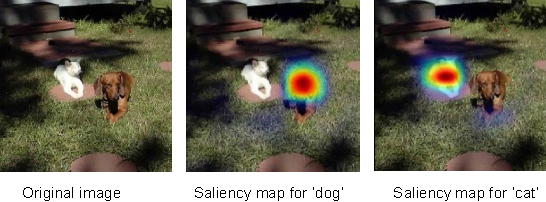
\includegraphics[width=0.80\linewidth]{Bishop10_15}
  \end{center}
  \vspace{-0.2em}
  \figcap[0.97]{Grad-CAM for VGG-16: the same image, and the regions
  that decide `dog' and `cat' respectively. Bishop \& Bishop (2024),
  Fig.~10.15, from Selvaraju et al.\ (2016).}
\end{frame}

\begin{frame}{Turning the gradient against the network}
  \vspace{-0.45em}
  \begin{defx}[Fast gradient sign method]\label{th:fgsm}
    \small
    With the network fixed and $E(\mathbf{x}, t)$ its error on image
    $\mathbf{x}$ with true label $t$, move every pixel by $\epsilon$ in the
    direction that increases the error:
    \[
      \mathbf{x}' = \mathbf{x} + \epsilon\, \mathrm{sign}\big( \nabla_{\mathbf{x}} E(\mathbf{x}, t) \big).
    \]
  \end{defx}
  \vspace{-0.2em}
  \begin{propx}[Why a tiny $\epsilon$ is enough]\label{th:linear}
    \small
    For an activation linear in the pixels,
    $a = \mathbf{w}^{\mathsf T}\mathbf{x} + b$, the attack changes it by
    $\epsilon \|\mathbf{w}\|_1$: one step of $\epsilon$ per pixel, added
    over all $d$ of them, so it grows like $d$ while no single pixel
    changes by more than $\epsilon$. Training moves the parameters to
    reduce $E$; the attack moves the image to increase it, by the same
    backpropagation.
  \end{propx}
  \vspace{-0.3em}
  \srcline{Bishop \& Bishop (2024), \S10.3.4, Eq.~10.11;
  Goodfellow et al.\ (2014).}
\end{frame}

\begin{frame}{What the attacks show}
  \vspace{-0.2em}
  {\footnotesize
  \begin{itemize}\itemsep0.16em
    \item An imperceptible change makes a network misclassify with
          high confidence
    \item Not over-fitting: an image adapted to fool one network fools
          others, and a \alert{linear} model is fooled the same way ---
          Proposition~\ref{th:linear} is the reason
    \item Physical objects can be built that a plain photograph of
          misclassifies; simple attacks yield to simple changes in
          training, sophisticated ones are an open problem
  \end{itemize}}
  \vspace{-0.2em}
  \begin{center}
    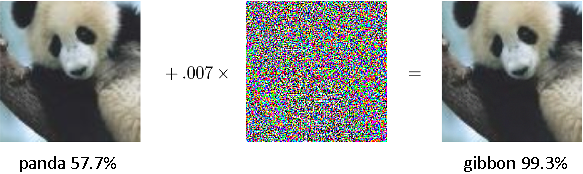
\includegraphics[height=0.19\textheight]{Bishop10_16}\hspace{1.2em}%
    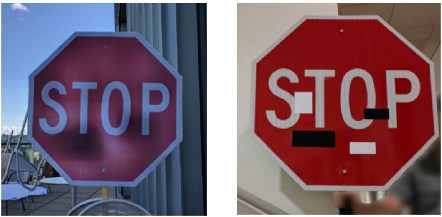
\includegraphics[height=0.19\textheight]{Bishop10_17}%
  \end{center}
  \vspace{-0.7em}
  {\tiny\color{mcMuted}
  Left: panda $57.7\%$ $\to$ gibbon $99.3\%$. Right: stop signs read as
  $45$\,mph. \hfill Bishop \& Bishop (2024), Figs.~10.16--10.17, from
  Goodfellow et al.\ (2014) and Eykholt et al.\ (2018).\par}
\end{frame}

\begin{frame}{DeepDream: amplify what a layer already sees}
  \vspace{-0.3em}
  \begin{defx}[DeepDream]\label{th:dream}
    \small
    Forward-propagate an image $I$ to a chosen layer, set each unit's
    $\delta$ there equal to its own pre-activation, backpropagate to
    the pixels, and step the image along the gradient. This ascends
    \[
      F(I) = \sum_{i, j, k} a_{ijk}(I)^2 ,
    \]
    the sum of squared pre-activations of the layer.
  \end{defx}
  \vspace{0.1em}
  {\footnotesize
  \begin{itemize}\itemsep0.22em
    \item Whatever the layer responds to a little is made to respond
          a lot: a cat-like cloud becomes more cat-like, over several
          iterations, with smoothing and clipping to keep it plausible
    \item From noise it makes an image entirely of the network's own
  \end{itemize}}
  \vspace{-0.3em}
  \srcline{Bishop \& Bishop (2024), \S10.3.5, Eq.~10.12, Exercise 10.10;
  Mordvintsev et al.\ (2015).}
\end{frame}

\begin{frame}{DeepDream, on an image}
  \begin{center}
    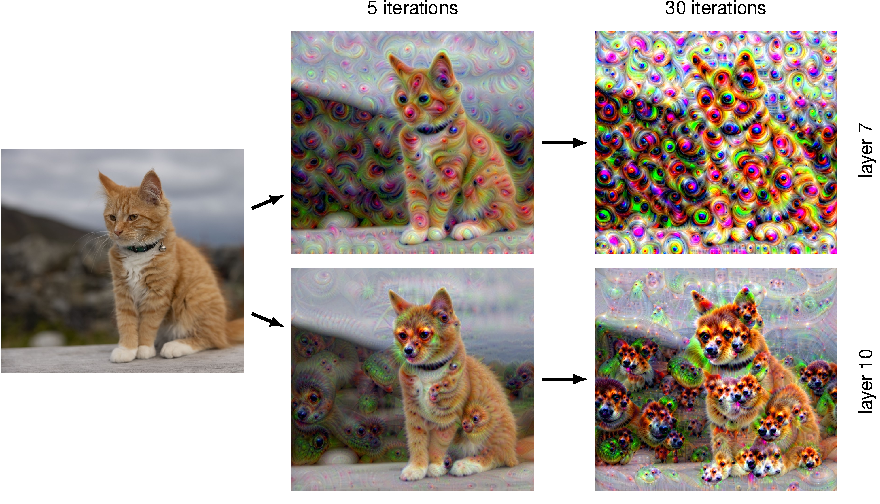
\includegraphics[width=0.62\linewidth]{Bishop10_18}
  \end{center}
  \vspace{-0.2em}
  \figcap[0.97]{Layer 7 (top) and layer 10 (bottom) of VGG-16, after
  five and thirty iterations. Bishop \& Bishop (2024), Fig.~10.18.}
\end{frame}

% =====================================================================
\section{Style Transfer}
% =====================================================================

\begin{frame}{Content and style, as errors}
  \vspace{-0.3em}
  \begin{defx}[Neural style transfer]\label{th:style}
    \small
    Generate $G$ from a content image $C$ and a style image $S$ by
    descent on $E(G) = E_{\mathrm{content}}(G, C) + E_{\mathrm{style}}(G, S)$,
    at a convolutional layer with $I \times J$ maps and $K$ channels:
    \[
      E_{\mathrm{content}} = \sum_{i,j,k} \big\{ a_{ijk}(G) - a_{ijk}(C) \big\}^2,
      \quad
      F_{kk'} = \sum_{i,j} a_{ijk}\, a_{ijk'},
      \quad
      E_{\mathrm{style}} = \frac{\sum_{k,k'} \{ F_{kk'}(G) - F_{kk'}(S) \}^2}{(2IJK)^2}.
    \]
  \end{defx}
  \vspace{-0.1em}
  {\footnotesize
  \begin{itemize}\itemsep0.16em
    \item Content is matched \emph{feature by feature, in place}; style
          through the $K \times K$ \alert{style matrix} of co-occurrences,
          summed over every location; in practice
          $\sum_l \lambda_l E^{(l)}_{\mathrm{style}}$ over several layers
  \end{itemize}}
  \srcline{Bishop \& Bishop (2024), \S10.6, Eqs.~10.13--10.17;
  Gatys et al.\ (2015).}
\end{frame}

\begin{frame}{Why the style matrix forgets position}
  \vspace{-0.45em}
  \begin{propx}[The style matrix is translation-invariant]\label{th:gram}
    \small
    Translating every feature map by the same amount leaves
    $F_{kk'} = \sum_{ij} a_{ijk} a_{ijk'}$ unchanged, up to the values
    that leave the frame, since the sum runs over all positions and a
    translation only permutes them. The content error has no such
    invariance: it compares position with position.
  \end{propx}
  \vspace{0.05em}
  {\footnotesize
  \begin{itemize}\itemsep0.26em
    \item \focus{1}{Proof. Write $a'_{ijk} = a_{i+u,\,j+v,\,k}$. Then
          $\sum_{ij} a'_{ijk} a'_{ijk'} = \sum_{ij} a_{i+u,j+v,k}\,
          a_{i+u,j+v,k'}$, a re-indexing of the same sum over the
          positions that stay inside. \hfill $\square$}
    \item \focus{2}{So $F$ measures whether a vertical edge tends to
          come with an orange blob, \emph{wherever} the two are ---
          which is what one means by the style of a painting.}
    \item \focus{3}{Early layers match edges; later layers match larger
          structures. The layer chosen decides how literal the copy is.}
  \end{itemize}}
  \vspace{-0.3em}
  \srcline{Bishop \& Bishop (2024), \S10.6.}
\end{frame}

\begin{frame}{Style transfer, on an image}
  \begin{center}
    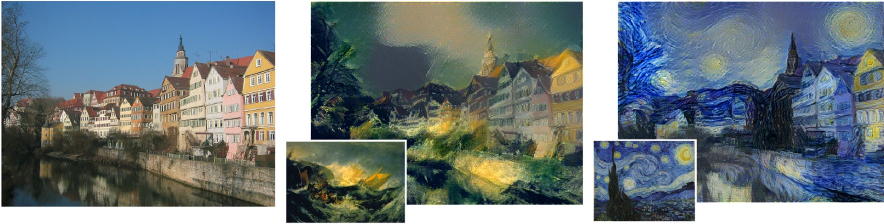
\includegraphics[width=0.94\linewidth]{Bishop10_32}
  \end{center}
  \vspace{-0.2em}
  \figcap[0.97]{A canal scene (left) rendered in the style of Turner's
  \emph{The Wreck of a Transport Ship} (centre) and of van Gogh's
  \emph{The Starry Night} (right); the style image is inset. Bishop \&
  Bishop (2024), Fig.~10.32, from Gatys et al.\ (2015).}
\end{frame}

% =====================================================================
\section{Putting It Together}
% =====================================================================

\begin{frame}{One gradient, five uses}
  \vspace{0.2em}
  {\scriptsize
  \renewcommand{\arraystretch}{1.36}
  \begin{tabular}{@{}l@{\hspace{1.0em}}l@{\hspace{1.0em}}l@{\hspace{1.0em}}l@{}}
    \textbf{Use} & \textbf{Differentiate} & \textbf{With respect to} & \textbf{Then}\\
    training & the error & the parameters & descend\\
    synthetic images & a class pre-activation & the pixels & ascend, regularised\\
    saliency & a class pre-activation & the last conv layer & average, weight, overlay\\
    adversarial attack & the error & the pixels & one signed step of $\epsilon$\\
    DeepDream & $\sum a_{ijk}^2$ at a layer & the pixels & ascend, repeat\\
    style transfer & content $+$ style error & the pixels of $G$ & descend from noise\\
  \end{tabular}}
  \vspace{0.6em}

  \begin{redhighlight}
    Backpropagation does not care which end of the network it stops at.
    Everything in the second half of today is Class 11's algorithm with
    the image, not the weights, as the variable.
  \end{redhighlight}
\end{frame}

\begin{frame}{Takeaways}
  \vspace{-0.1em}
  {\scriptsize
  \begin{enumerate}\itemsep0.22em
    \item A layer with channels has $(M^2 C_{\mathrm{in}} + 1) C_{\mathrm{out}}$
          parameters; stacking small kernels reaches as far as a large
          one for far fewer (Definition~\ref{th:layer})
    \item Two linear kernels are one kernel; the ReLU between them is
          what makes depth more than a factorisation
          (Proposition~\ref{th:compose})
    \item Simple cells are Gabor filters (Definition~\ref{th:gabor}),
          and so, to the eye, are a trained first layer --- because of
          image statistics, not because the network is a brain
    \item Deeper units are read by what excites them: edges, textures,
          parts, objects; or by ascending the pre-activation
          (Proposition~\ref{th:preact})
    \item Grad-CAM weights the last convolutional layer by averaged
          gradients (Definition~\ref{th:gradcam})
    \item One signed step of $\epsilon$ per pixel fools a network, and
          fools a linear model for a linear reason
          (Definition~\ref{th:fgsm}, Proposition~\ref{th:linear})
    \item Style is the co-occurrence of features summed over position,
          which is why the style matrix forgets where
          (Definition~\ref{th:style}, Proposition~\ref{th:gram})
  \end{enumerate}}
  \vspace{-0.2em}
  \bridge{Next: why the deepest trunks stop training well, and the
  residual connection that fixes it.}
\end{frame}

\begin{frame}[allowframebreaks]{References}
  \vspace{0.3em}
  {\scriptsize
  \begin{enumerate}\itemsep0.30em
    \item C.\ M.\ Bishop \& H.\ Bishop, \emph{Deep Learning: Foundations
          and Concepts}, Springer, 2024. \S10.2.7--10.2.8
          (Figs.~10.9--10.10, Exercise 10.8); \S10.3 (Eqs.~10.6--10.12,
          Figs.~10.11--10.18); \S10.6 (Eqs.~10.13--10.17, Fig.~10.32).
    \item S.\ J.\ D.\ Prince, \emph{Understanding Deep Learning}, MIT
          Press, 2023. \S10.5.1, Fig.~10.14.
    \item D.\ H.\ Hubel \& T.\ N.\ Wiesel, ``Receptive fields of single
          neurones in the cat's striate cortex'', \emph{J.\ Physiology}
          148, 1959.
    \item K.\ Fukushima, ``Neocognitron'', \emph{Biological
          Cybernetics} 36, 1980.
    \item Y.\ LeCun et al., ``Backpropagation applied to handwritten
          zip code recognition'', \emph{Neural Computation} 1(4), 1989.
    \item A.\ Krizhevsky, I.\ Sutskever \& G.\ E.\ Hinton, ``ImageNet
          classification with deep convolutional neural networks'',
          NeurIPS 2012.
    \item K.\ Simonyan \& A.\ Zisserman, ``Very deep convolutional
          networks for large-scale image recognition'', ICLR 2015.
    \item A.\ Hyv\"arinen, J.\ Hurri \& P.\ O.\ Hoyer, \emph{Natural
          Image Statistics}, Springer, 2009.
    \item M.\ D.\ Zeiler \& R.\ Fergus, ``Visualizing and understanding
          convolutional networks'', ECCV 2014 (arXiv 2013).
    \item J.\ Yosinski et al., ``Understanding neural networks through
          deep visualization'', ICML Deep Learning Workshop, 2015.
    \item R.\ R.\ Selvaraju et al., ``Grad-CAM: visual explanations from
          deep networks via gradient-based localization'', ICCV 2017
          (arXiv 2016).
    \item I.\ J.\ Goodfellow, J.\ Shlens \& C.\ Szegedy, ``Explaining and
          harnessing adversarial examples'', ICLR 2015 (arXiv 2014).
    \item K.\ Eykholt et al., ``Robust physical-world attacks on deep
          learning visual classification'', CVPR 2018.
    \item A.\ Mordvintsev, C.\ Olah \& M.\ Tyka, ``Inceptionism: going
          deeper into neural networks'', Google Research Blog, 2015.
    \item L.\ A.\ Gatys, A.\ S.\ Ecker \& M.\ Bethge, ``A neural
          algorithm of artistic style'', arXiv:1508.06576, 2015.
  \end{enumerate}}
\end{frame}

\begin{frame}[standout]
  Questions?
\end{frame}

\end{document}
